% !TeX spellcheck = en_GB

\section{Theoretical Aspects of Dendritic Computation}
\label{sec:dendritic_computation_theory}

\begin{figure}
	\centering
	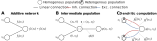
\includegraphics{media/chapters/03_nlif/03_01/nef_multivariate_functions.pdf}%
	{\phantomsubcaption\label{fig:nef_multivariate_functions_a}}%
	{\phantomsubcaption\label{fig:nef_multivariate_functions_b}}%
	{\phantomsubcaption\label{fig:nef_multivariate_functions_c}}%
	\caption[Using dendritic computation to compute multivariate functions in the NEF]{Using dendritic computation to compute multivariate functions in the NEF. \textbf{(A)} Standard NEF networks are additive: summation in activity space corresponds to addition in representation space.
	\textbf{(B)} Computing nonlinear multivariate functions $\phi$ generally requires all variables to be represented in an intermediate population.
	\textbf{(C)} The dendritic computation scheme discussed in here.
	Two pre-populations project onto a post-population with separate excitatory and inhibitory input channels.
	%The nonlinear interaction between these channels is exploited to compute $\phi$.
	}
	\label{fig:nef_multivariate_functions}
\end{figure}

The idea of dendritic computation as pursued here is best explained by reviewing fundamental properties of neural networks, and exploring how mul\-ti\-va\-ri\-ate functions such as $f(x_1, \ldots, x_\ell)$ can be computed in the NEF.
Specifically, we analyse three different network architectures (cf.~\Cref{fig:nef_multivariate_functions}).
\emph{Additive networks} represent $x_1$, $\ldots$, $x_\ell$ in independent neuron populations.
These networks cannot approximate most multivariate functions.
In contrast, \emph{two-layer networks} can represent all variables in a common intermediate population.
These networks are universal approximators.
Lastly, our notion of \emph{dendritic computation} relies on non-linear interaction between independent neural input channels.
While not as powerful as multi-layer networks, dendritic computation can approximate a larger class of functions well compared to additive networks.

\subsection{Additive Multivariate Networks}
\label{sec:additive_net}

As stated above, our goal is to compute multivariate functions $f(x_1, \ldots, x_\ell)$ within the context of the NEF.
%For the sake of simplicity, we mostly discuss bivariate functions of the form $\phi(x_1, x_2)$, but the same considerations apply to more than two input variables as well.
For the sake of simplicity, assume that two pre-populations representing the variables $x_1$, $x_2$ are connected to a common post-population.
To compute $f(x_1, x_2)$, we must find connection weights $\vec w_{1, i}$, $\vec w_{2, i}$ such that the following holds for every post-neuron $i$
\begin{align}
	a_i(f(x_1, x_2))
		= G_i \bigl[
			\langle \vec e_i, f(x_1, x_2) \rangle
		\bigr]
		\supposedEq G_i\bigl[
			\langle \vec w_{1, i}, \vec a^\mathrm{pre}_1(x_1) \rangle + \langle \vec w_{2, i}, \vec a^\mathrm{pre}_2(x_2)
		\rangle\bigr] \,.
	\label{eqn:nef_multivariate_addition}
\end{align}
Here, $a_i$ is the desired post-neuron activity according to the normative tuning-curve constraint (eq.~\ref{eqn:encoding}).
As discussed in the context of the NEF transformation principle (cf.~\Cref{sec:nef_transformation}), we assume that the current-translation function $J_i$ is part of the individual neuron response curve $G_i$, and that the currents induced by the pre-populations are summed.

Now, consider multivariate functions that can be decomposed into a sum of two univariate functions, i.e., $f(x_1, x_2) = f_1(x_1) + f_2(x_2)$ (cf.~\Cref{fig:nef_multivariate_functions_a}).
We can easily find weights $\vec w_{1, i}$, $\vec w_{2, i}$ that approximate $f$ using the encoder-decoder split of the NEF \citep[cf.][Section~6.1.2]{eliasmith2003neural}.
Computing decoders $\mat D^{f_1}$, $\mat D^{f_2}$ and applying $(\vec w_i)^T = \vec e_i \mat D$, we have
\begin{align*}
	G_i\bigl[
	  \langle
	  	\vec e_i \mat D^{f_1},
	  	\vec a^\mathrm{pre}_1(x_1)
	  \rangle
	+ \langle
	  	\vec e_i \mat D^{f_2},
		\vec a^\mathrm{pre}_2(x_2)
	\rangle\bigr] = 
	G_i\bigl[\langle \vec e_i, \mat D^{f_1} \vec a_1^\mathrm{pre}(x_1) + \mat D^{f_2} \vec a_2^\mathrm{pre}(x_2) \rangle\bigr]
	\approx a_i\bigl(f_1(x_1) + f_2(x_2)\bigr) \,.
\end{align*}
This equation expresses that addition in activity space (i.e., summing weighted pre-activities, eq.~\ref{eqn:nef_multivariate_addition}) is equal to addition in represented space.
In other words, standard NEF networks are \emph{additive}.
Summing functions incurs no additional decoding error.

\begin{figure}
	\centering
	
\includegraphics{media/chapters/03_nlif/03_01/perceptron.pdf}%
	{\phantomsubcaption\label{fig:perceptron_a}}%
	{\phantomsubcaption\label{fig:perceptron_b}}%
	\caption[Additive networks are a generalisation of the perceptron]{Additive networks are a generalisation of the perceptron. \textbf{(A)} An additive network is a sum of arbitrary univariate functions. \textbf{(B)} A perceptron is an additive network with functions of the form $f_i(x_i) = w_i x_i + \beta \ell^{-1}$. The weights $w_i$ are learned such that the output approximates a desired function.}
\end{figure}

\subsubsection{Additive networks cannot compute most multivariate functions}
The only way to compute general multivariate functions $f(x_1, x_2)$ in additive networks is to \emph{approximate} $f$ as an additive univariate decomposition.
As is expressed by the following proposition (see Appendix~B.3.1 for a proof), it is impossible to compute many continuous multi-variate $f$ using such additive networks.%
\footnote{We our propositions to continuous functions for the sake of simplicity.
However, we conjecture that the same results hold for larger classes of functions, for example square Lebesgue integrable functions.}
This is true even if we can decode arbitrary univariate functions $f_1$, $\ldots$, $f_\ell$ over the pre-variables (this is equivalent to having an infinite number of pre-neurons, see below), and we were able to freely choose a fixed nonlinearity $\sigma$ (cf.~\Cref{fig:perceptron_a}).

\begin{restatable}{theorem}{ThmXorGeneral}
\label{thm:xor_general}
Let $\ell > 1$, $\Xrepr \subset \mathbb{R}^\ell$ and $\mathbb{Y} \subset \mathbb{R}$ be compact sets of full dimensionality, and $\sigma$, $f$, $f_i$ be continuous.
For any fixed $\sigma : \mathbb{R} \longrightarrow \mathbb{Y}$, there always exist $f : \Xrepr \longrightarrow \mathbb{Y}$ such that there is no $f_1$, $\ldots$, $f_\ell : \mathbb{R}  \longrightarrow \mathbb{R}$ with
$f(x_1, \ldots, x_\ell) = \sigma\bigl( f_1(x_1) + \ldots + f_\ell(x_\ell) \bigr)$ for all $(x_1, \ldots, x_\ell) \in \Xrepr$.
\end{restatable}

\begin{figure}
	\centering
	\includegraphics{media/chapters/03_nlif/03_01/xor_visualisation.pdf}%
	{\phantomsubcaption\label{fig:xor_visualisation_a}}%
	{\phantomsubcaption\label{fig:xor_visualisation_b}}%
	{\phantomsubcaption\label{fig:xor_visualisation_c}}%
	{\phantomsubcaption\label{fig:xor_visualisation_d}}%
	{\phantomsubcaption\label{fig:xor_visualisation_e}}%
	\caption[Visualisation of the XOR decision problem for different classifiers]{Visualisation of the XOR decision problem for different classifiers. The goal is to find classifier parameters such that the four samples are classified as depicted.
	The background corresponds to the sign of the monotonic function $\sigma(\xi)$.
	\textbf{(A)} The linear decision boundary formed by the Perceptron cannot solve the XOR problem.
	\textbf{(B)} This holds for any function of the form $\sigma(f_1(x_1) + f_2(x_2))$, here $f_1(x_1) = \cos(2\pi x_1)$ and $f_2(x_2) = \sin(2\pi x_2)$.
	\textbf{(C)} A multi-layer Perceptron (MLP) of the form $\sum_i w_i \sigma(e_i^1 x_1 + e_i^2 x_2 + \beta_i )$ can solve the problem, although the decision boundary is quite erratic.
	\textbf{(D)} An alternative solution using the nonlinearity $\sigma'(\xi) = \sigma(\xi^2 - 1)$.
	\textbf{(E)} Multiplication of two real-valued variables $x_1$, $x_2$ can be seen as a continuous form of the XOR problem.
	Additive networks cannot compute this function.
	}
	\label{fig:xor_visualisation}
\end{figure}

\subsubsection{The Perceptron and XOR}
Consider monotonic $\sigma$ and affine $f_i$ of the form $w_i x_i + \beta \ell^{-1}$.
We obtain the \emph{perceptron}, an early single-layer neural network (cf.~\Cref{fig:perceptron_b}; \cite{rosenblatt1958perceptron}).
\Citet[Chapter~2; originally published in 1969]{minsky1987perceptrons} point out that such networks cannot compute the boolean XOR function (\Cref{fig:xor_visualisation_a}).%
\footnote{\Citet{minsky1987perceptrons} note that the perceptron was proved by Rosenblatt to \enquote{learn to do anything it was possible to program it to do}; this ambiguous statement endowed researchers with a surplus of optimism---especially since perceptrons sometimes learned difficult problems.
Among other factors, realising that these networks could not be \emph{programmed} to solve trivial problems such as XOR led to \enquote{the first AI winter} \citep[e.g.,][]{muthukrishnan2020brief}.}
%In the continuous domain, the same is true for multiplication over $\mathbb{X} = [-1, 1]^2$, that is $\phi(x_1, x_2) = x_1 x_2$ (\Cref{fig:xor_visualisation_a}).
Even the general additive networks from our theorem cannot solve a \emph{weaker} version of the XOR problem, formalised below.

\begin{definition}
\label{def:weak_xor}
A function $\phi(x_1, x_2)$ solves the \emph{weak XOR problem} if there exist $a_0, b_0, a_1, b_1$ with
\begin{align*}
	\big( \phi(a_0, b_0) < \phi(a_0, b_1) \big) \wedge
	\big( \phi(a_1, b_1) < \phi(a_0, b_1) \big) \wedge
	\big( \phi(a_0, b_0) < \phi(a_1, b_0) \big) \wedge
	\big( \phi(a_1, b_1) < \phi(a_1, b_0) \big) \,.
\end{align*}
\end{definition}

%That is, we merely require $\phi(a_0, b_0)$ and $\phi(a_1, b_1)$ to be larger than $\phi(a_0, b_1)$ and $\phi(b_1, b_0)$.

\begin{restatable}{theorem}{ThmWeakXor}
\label{thm:weak_xor}
Let $\sigma$ be monotonic. Then, an additive network of the form $\phi(x_1, x_2) = \sigma(f_1(x_1) + f_2(x_2))$ cannot solve the weak XOR problem.
\end{restatable}
This may be surprising, given that, as depicted in \Cref{fig:xor_visualisation_b}, we can generate highly nonlinear classification boundaries.
We provide a proof in Appendix~B.3.2.

To solve the XOR problem, we can either, as discussed next, use multi-layer networks (cf.~\Cref{fig:xor_visualisation_c}), or, alternatively make $\sigma$ non-monotonic.
As depicted in \Cref{fig:xor_visualisation_d}, setting $\sigma(\xi) = \xi^2 - 1$ allows us to solve the XOR problem.
This illustrates our goal with dendritic computation: exploit \enquote{more powerful} $\sigma$ to approximate a larger class of functions.

Still, the functions that we can compute using additive networks are limited, even if we can freely choose $\sigma$.
For example, we can compute $x_1 x_2$ for $(x_1, x_2) \in [\epsilon, 1]^2$ and $0 < \epsilon < 1$ by setting $f_1$ and $f_2$ to the logarithm and $\sigma$ to the exponential.
However, it is impossible to find functions that compute multiplication over all four quadrants---which can be seen as a continuous version of the XOR problem (\Cref{fig:xor_visualisation_e}).
More precisely, allowing $x_1$, $x_2$ to be zero makes it impossible to compute multiplication in these networks (proof in Appendix~B.3.3).
\begin{restatable}{theorem}{ThmMultiplication}
\label{thm:multiplication}
There are no continuous, real-valued functions $f_1$, $f_2$, $\sigma$ such that $\sigma(f_1(x_1) + f_2(x_2)) = x_1 x_2$ for all $(x_1, x_2) \in [0, 1]^2$.
\end{restatable}


%Choosing this $\sigma$ implicitly introduces a non-linear interaction between the variables $x_1$, $x_2$, for example
%\begin{align*}
%	\sigma\left( (w_1 x_1 + w_2 x_2 + \beta)^2 - 1\right) = 
%	\sigma\left( w_1^2 x_1^2 + w_2^2 x_2^2 + 2 w_1 w_2 x_1 x_2 + 2 w_1 \beta x_1 + 2 w_2 \beta x_2 + \beta^2  - 1\right) \,.
%\end{align*}
%The product-term $w_1 w_2 x_1 x_2$ can be exploited to %compute multiplication-like functions.
%Still, as stated in Theorem~1, there inevitably is a large set of functions that we cannot compute.
% TODO Add reference

\subsection{Two-Layer Networks and Intermediate Populations}

\begin{figure}
	\includegraphics{media/chapters/03_nlif/03_01/mlp.pdf}
	\caption[Sketch of a two-layer neural network]{Sketch of a two-layer neural network with rectified linear units (ReLUs). If the encoding vectors $\vec e_i$ and the biases $\beta_i$ are sampled appropriately, this network is a universal function approximator.}
	\label{fig:mlp}
\end{figure}

As already mentioned in \Cref{sec:nef_transformation}, an individual NEF population can be interpreted as a two-layer neural network (cf.~\Cref{fig:mlp}).
As long as the encoding vectors are sampled from the $\ell$-dimensional hypersphere and $x$-intercepts are uniformly distributed, such a neuron population is a universal function approximator, that is, we can compute arbitrary functions $f(x_1, \ldots, x_\ell)$ over the variables represented in the population.
The following theorem states this more formally for neurons with a rectified linear unit (ReLU) nonlinearity, i.e., $\sigma(\xi) = \max\{0, \xi\}$.

\begin{restatable}{theorem}{ThmTwoLayerUniversal}
\label{thm:two_layer_universal}
Let $\ell \geq 1$, and $f : \mathbb{B}^\ell \longrightarrow \mathbb{R}$ be a continuous function mapping from the $\ell$-dimensional unit ball onto $\mathbb{R}$.
Furthermore, let $\sigma(\xi) = \max\{0, \xi\}$, $\vec e_i$ be sampled uniformly from the unit-sphere $\mathbb{S}^\ell$, and $\alpha_i$ and $\beta_i$ be sampled such that $-\beta_i / \alpha_i$ is uniformly distributed between $[-1, 1]$ and $\alpha_i + \beta_i$ is uniform over $(0, 1]$.
There exist $d_i \in \mathbb{R}$ such that
\begin{align}
	\vspace*{-0.5em}
	f(\vec x) = \lim_{\Npop \to \infty} \sum_{i = 1}^{\Npop} d_i \sigma\bigl( \alpha_i \langle \vec e_i, \vec x \rangle + \beta_i \bigr) \quad \text{for all} \quad \vec x \in \mathbb{B}^\ell \,.
	\label{eqn:two_layer_network}
\end{align}
\end{restatable}
\vspace*{-0.5em}\noindent
This follows directly from \citet{hornik1989multilayer}.
We provide a more thorough discussion \Cref{app:thm_two_layer_universal}.
This theorem can be extended to hold for arbitrary compact domains $\Xrepr$, codomain dimensionalities, and other neural nonlinearities $\sigma$.

%It may not be obvious why \cref{eqn:two_layer_network} describes a \enquote{two-layer} neural network.
%In essence, the encoding weights $\vec e_i$ map $\vec x$ onto the input of one of the $N$ neurons with nonlinearity $\sigma$.
%This step forms the \enquote{first} or \enquote{hidden layer}.
%The decoding weights $d_i$ then map the neural activities $\sigma(\xi_i)$ onto the output, which forms the \enquote{second layer} (cf.~Figure~2.20).
%% TODO: Add actual reference

\subsubsection{The role of uniformly sampled encoders}
Theorem~\ref{thm:two_layer_universal} requires that the encoding vectors $\vec e_i$ are uniformly sampled from the hypersphere $\mathbb{S}^\ell$.%
\footnote{There are weaker requirements for specific $f$.
As demonstrated by \citet{gosmann2015precise} in the context of multiplication, there are certain distributions of encoding vectors that minimise the decoding error.
Global optimisation methods such as stochastic gradient descent systematically select such \enquote{optimal} encoders.}
To see why this is important, consider the case where the $\vec e_i$ are axis-aligned, i.e., $\|\vec e_i\|_0 = 1$ (cf.~Appendix~A.1).
% TODO: Add reference for zero-norm in Appendix~A.1
In this case, we can split \cref{eqn:two_layer_network} into $\ell$ sub-networks, each decoding a function over a single variable $x_\ell$
\begin{align*}
		\sum_{i = 1}^N d_i \sigma\bigl( \langle \vec e_i, \vec x \rangle - \beta_i \bigr)
	= 	\sum_{j = 1}^\ell \sum_{i = 1}^{N_j} d_{j i} \sigma\bigl( e_{j i} x_j - \beta_{j i} \bigr) \,, \text{where } e_{j i} \in \{ -1, 1\} \,.
\end{align*}
This is equivalent to the additive networks we discussed before.
We can only decode sums of univariate functions over the individual $x_j$ from the pre-population.

\subsubsection{Intermediate populations}
%We now know that we can indeed approximate multivariate functions in the NEF with an arbitrarily small error.
%The pre-condition for this is that all variables over which we would like to compute a $\phi$ represented in the same neuron population with non-axis aligned encoding vectors $\vec e_i$.
As discussed by \citep[Chapter~6]{eliasmith2003neural}, multivariate functions $f(x_1, x_2)$ can in general only be computed if all variables $x_1$, $x_2$ are represented in a common intermediate population.
Correspondingly, this intermediate population represents a vectorial quantity $\vec z = (x_1, x_2)$ (cf.~\Cref{fig:nef_multivariate_functions_b}).
We can construct such a representation from two univariate populations by computing the functions $f_1(x_1) = (x_1, 0)$ and $f_2(x_2) = (0, x_2)$ in the connections to the intermediate population.
According to Theorem~\ref{thm:two_layer_universal} we can then decode any multivariate function from the intermediate population.

\subsubsection{Potential issues with intermediate populations}
In theory, the number of neurons required to cover a $d$-dimensional space rises exponentially with $d$.
Representing a $d$-dimensional quantity in an intermediate population thus requires many neurons to achieve a certain decoding error for all target functions.
In practice, it is quite difficult to judge the number of neurons required to decode a certain function $f$ a-priori; the decoding error heavily depends on $f$ and the encoding vectors $\vec e_i$.

Another problem arises when modelling neurobiological systems.
There may be no indication that an intermediate population exists in a particular biological circuit, but the function can be modelled well as a multivariate function.
An example of this would be the aforementioned attention system, where a group of control neurons modulates another population without an intermediary \citep{bobier2014unifying}.

Finally, there is the issue of noise.
In spiking neural networks, every intermediate neuron population introduces additional noise due to static distortion and spike noise \citep[Section~2.2.2]{eliasmith2003neural}.
We see the effects of this later.

\subsection{Dendritic Computation}
\label{sec:dendritic_computation_theory_dendritic}

Dendritic computation is one way to partially alleviate the limitations arising from intermediate populations.
The basic idea is that each neuron possesses $k$ \emph{input channels}.
Input fed through these channels interacts nonlinearly, modelling information processing within the dendrites.

\begin{figure}
	\includegraphics{media/chapters/03_nlif/03_01/dendritic_computation.pdf}%
	{\phantomsubcaption\label{fig:dendritic_computation_net}}%
	{\phantomsubcaption\label{fig:dendritic_computation_fun}}%
	\caption[Overview of our notion of dendritic computation.]{Overview of our notion of dendritic computation. \textbf{(A)} Neuron with an excitatory and inhibitory input channel. In a network context, these functions are decoded from pre-populations representing these variables. Connectivity can be constrained such that excitatory and inhibitory pre-neurons only connect to the corresponding channel. \textbf{(B)} Conceptually, each channel receives a sum of univariate functions computed over the pre-variables $x_1$, $\ldots$, $x_\ell$.}
\end{figure}

Mathematically, the response curve describing the average neural activity is now a multivariate function $\mathscr{G}[\xi_1, \ldots, \xi_k]$, where the $\xi_i$ are linear combinations of the pre-activities (\Cref{fig:dendritic_computation_net}).
To compute $\phi(x_1, \ldots, x_\ell)$, the following must hold for each post-neuron $i$
\begin{align}
	\begin{aligned}
	a_i\bigl(\phi(x_1, \ldots, x_\ell)\bigr) &\supposedEq
	\mathscr{G} \bigl[
		\langle \vec w_{1, i}^1, \vec a^\mathrm{pre}_1(x_1) \rangle + \ldots +
		\langle \vec w_{\ell, i}^1, \vec a^\mathrm{pre}_\ell(x_\ell) \rangle, \ldots,\\
%	&~\quad\quad\vdots, \\
	&~\hspace{1.66em}
		\langle \vec w_{1, i}^k, \vec a^\mathrm{pre}_1(x_1) \rangle + \ldots +
		\langle \vec w_{\ell, i}^k, \vec a^\mathrm{pre}_\ell(x_\ell) \rangle
	\bigr]
	\end{aligned}
	\label{eqn:dendritic}
\end{align}
where $a_i(\phi(x_1, \ldots, x_\ell))$ expresses the normative tuning constraint defined in \cref{eqn:encoding}.

Note that we deliberately left the concept of an \enquote{input channel} open.
An input channel could either refer to a different location in the dendritic tree, different synapse types (e.g., excitatory or inhibitory synapses), or even the influence of other signalling molecules.
We discuss examples of model neurons with multiple input channels in \Cref{sec:nlif}.

\subsubsection{Mathematical analysis}
More formally, using $\sigma(\xi_1, \ldots, \xi_\ell)$ as an abstract nonlinearity and assuming that we can compute any univariate function $g_i^j$ over $\xi_1, \ldots, \xi_\ell$, we have (\Cref{fig:dendritic_computation_fun})
\begin{align}
	\sigma \bigl(
		g_{1}^1(x_1) + \ldots + g_{\ell}^1(x_\ell), \ldots, g_{1}^k(x_1) + \ldots + g_{\ell}^k(x_\ell)
	\bigr) = \phi(x_1, \ldots, x_\ell) \,.
	\label{eqn:dendritic_computation_theory}
\end{align}
It is trivial to show that such networks are more powerful than additive networks.
For example, let $\sigma(\xi_1, \xi_2) = \xi_1 \xi_2$.
Now, setting the functions feeding into the second channel to one, i.e., $g_{1, i}^2(x_1) = \ldots = g_{\ell, 1}^2(x_\ell) = 1$, we obtain an additive network.
Of course, in contrast to additive networks, we can use the same $\sigma$ to compute products of the pre-variables.
Still, dendritic computation computation networks are not universal approximators:
\begin{conjecture}
\label{thm:dendritic_compuation_incomplete}
Let $\ell > 1$, $\Xrepr \subset \mathbb{R}^\ell$ and $\mathbb{Y} \subset \mathbb{R}$ be compact sets of full dimensionality, and $\sigma$, $f$, $g^j_i$ be continuous.
For any fixed $\sigma : \mathbb{R}^k \longrightarrow \mathbb{Y}$, there always exist $f : \Xrepr \longrightarrow \mathbb{Y}$ such that there are no $g^1_1, \ldots, g^1_\ell, \ldots, g^k_1, \ldots, g^k_\ell : \mathbb{R}  \longrightarrow \mathbb{R}$ with the property
\begin{align*}
	f(x_1, \ldots, x_\ell) = \sigma(\xi_1, \ldots, \xi_k) = \sigma\bigl( g^1_1(x_1) + \ldots + g^1_\ell(x_\ell), \ldots,  g^k_1(x_1) + \ldots + g^k_\ell(x_\ell)\bigr) \text{ for all } \vec x \in \Xrepr \,.
\end{align*}
\end{conjecture}
\noindent While we do not have a rigorous proof, counting the degrees of freedom (DOF) required to describe an $\ell$-dimensional function $f$ suggests that this should be true.
Given $\oh$ orthogonal one-dimensional basis functions, the corresponding $\ell$-dimensional basis has $\oh^\ell$ basis functions.
Correspondingly, $\oh^\ell$ DOF are required to describe an $\ell$-dimensional $f$ with a basis of order $\oh$.
However, when using dendritic computation, we only use $k \ell$ one-dimensional functions; correspondingly, there are only $\oh k \ell$ DOF.
For $\oh \to \infty$, and $\ell > 1$, $\oh k \ell$ grows much slower than $\oh^\ell$.
Hence, there are always functions than cannot be computed using dendritic computation.%
\footnote{Mathematically, the cardinality of the set of continuous functions $f$ constructed from a function basis of order $\oh$ is $|\mathbb{R}^{\oh^\ell}|$, while the cardinality of functions that can be constructed using dendritic computation is $|\mathbb{R}^{\oh k \ell}|$.
Unintuitively, even for $\oh \to \infty$, it holds $|\mathbb{R}^{\oh^\ell}| = |\mathbb{R}^{\oh k\ell}| = \mathfrak{c}$, where $\mathfrak{c}$ is the cardinality of the continuum \citep[e.g.,][Chapter~4]{jech2003set}.
Fortunately, this is irrelevant in practice.
Assuming some baseline precision and dynamic range of the generalised Fourier coefficients, there are only finitely many parameters $N$ that can be used to uniquely characterise each function. It clearly holds $N^{\oh^\ell} \gg N^{\oh k \ell}$ for $\ell > 1$ and $\oh \to \infty$.}

\subsection{Numerical Exploration}
\label{sec:dendritic_computation_theory_numerical}

The above discussion offers only limited insight into the practical implications of using dendritic computation.
The goal of this section is to provide a numerical analysis of our different network types.
Specifically, we characterise the \enquote{computational power} of a network by approximating two-dimensional functions $f(x_1, x_2)$ of varying complexity.
More \enquote{powerful} networks should be capable of computing \enquote{more complex} $f(x_1, x_2)$ at lower errors than other networks.
Since the \enquote{complexity} of a function is somewhat ill-defined, we use frequency content as a proxy.
Functions with a higher spatial bandwith contain more information \citep[cf.][]{shannon1949communication} than functions only composed of lower frequencies and should thus qualify as \enquote{more complex}.

\subsubsection{Generating random test functions}

\begin{figure}
	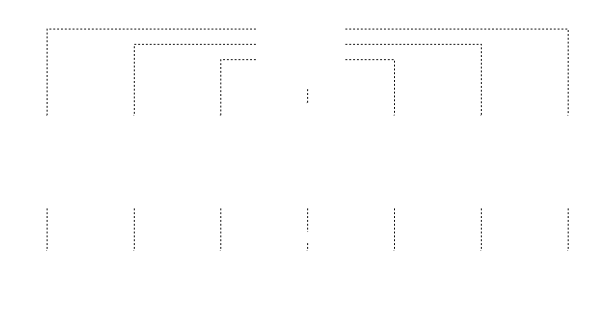
\includegraphics{media/chapters/03_nlif/03_01/2d_functions_overview_overlay.pdf}%
	\kern-157.24mm\includegraphics{media/chapters/03_nlif/03_01/2d_functions_overview.pdf}
	\caption[Overview of our procedure for generating random 2D functions]{Overview of our procedure for generating random 2D functions. \textbf{(A)} We sample a 2D array from a normal distribution (only a portion of the array is depicted; the size $n' \times n'$ depends on the filter width). \textbf{(B)} The noise is filtered by convolving with a Gaussian kernel with standard-deviation $\rho$ (for large filter widths, i.e., small $\rho^{-1}$, only a small portion of the filter is depicted). \textbf{(C)} The resulting functions are transformed to have mean zero (i.e., no DC component) and a standard deviation of one.}
	\label{fig:2d_functions_overview}
\end{figure}

To generate sampled random $f(x_1, x_2)$, we use the scheme depicted in \Cref{fig:2d_functions_overview}.
In a nutshell, we draw $n' \times n'$ points from a normal distribution and apply a 2D Gaussian filter with standard deviation $\rho$.
We then extract the desired $n \times n$ samples not affected by boundary effects, and normalise the result to zero mean and unit standard deviation.
As a result, small $\rho^{-1}$ (i.e., large filters), result in almost linear functions, whereas large $\rho^{-1}$ (small filters) result in high-frequency functions.%
\footnote{
Note that this scheme generates aperiodic functions.
Correspondingly, while the filtered grid of $n' \times n'$ samples is band-limited, the final $n \times n$ samples are not.
High frequencies are required to represent the discontinuous boundary---a result of applying a box-window to our data (cf.~the \enquote{windowing theorem}; e.g.,~\cite{oppenheim2009discretetime}, Section~2.9.7).
Hence, there is no trivial way to sample these functions directly the frequency domain, and to make use of the fast inverse Fourier transformation.
Still, this scheme can be implemented efficiently by separating the Gaussian filters into horizontal and vertical components \citep[e.g.][]{bolon2006twodimensional}.
}

\subsubsection{Network models}
To compare the above networks types, we could construct concrete networks and compare approximation errors for our randomly generated two-dimensional functions $\phi(x_1, x_2)$.
However, as a simplification, we can replace the pre-populations by the first $\oh$ Legendre polynomials $P_i(x)$.%
\footnote{We discuss of Legendre polynomials in Section~4.2. Note that we use a discretised version of the Legendre basis, \enquote{Discrete Legendre Orthogonal Polynomials} \citep[DLOPs;][]{neuman1974discrete,stockel2021discrete}.}
%TODO Reference to the Legendre polynomials
This is possible because the principal components of neural populations resemble Legendre polynomials \citep[Chapter~7]{eliasmith2003neural}.
Furthermore, using a function basis of order $\oh$ connects back to our previous theoretical discussion of dendritic computation in terms of degrees of freedom.
The number of basis functions that can be decoded well from a pre-population depends on the number of neurons in that population.
We explore this in more detail below.
%In a sense, thus we replace random neuron populations with the corresponding \enquote{optimal} orthogonal basis.

Replacing the pre-population in the additive network with $\oh$ basis functions, and under the assumption that $\sigma(\xi) = \xi$ (there is no additional nonlinearity), we get
\begin{align}
	f_\mathrm{add}(x_1, x_2) &= g_1(x_1) + g_2(x_2) = \sum\nolimits_{i = 0}^{\oh} w^1_{i} P_i(x_1) + \sum\nolimits_{i = 0}^{\oh} w^2_{i} P_i(x_2) \,,
	\label{eqn:f_add}
\end{align}
where $w_i^1$, $w_i^2$ (for $2o$ degrees-of-freedom; DOF) can be computed using least squares.
For our analysis of dendritic computation, we choose $\sigma(\xi_1, \xi_2) = \xi_1 \xi_2$ as a nonlinearity $\sigma$ and obtain
\begin{align}
	\begin{aligned}
		f_\mathrm{den}(x_1, x_2)
			&= \sigma\big(g^1_1(x_1) + g^1_2(x_2), g^2_1(x_1) + g^2_2(x_2)\big) \\
			&= \left( \sum\nolimits_{i = 0}^{\oh} w^1_{i} P_i(x_1) + \sum\nolimits_{i = 0}^{\oh} w^2_{i} P_i(x_2) \right)
			   \left( \sum\nolimits_{i = 0}^{\oh} w^3_{i} P_i(x_1) + \sum\nolimits_{i = 0}^{\oh} w^4_{i} P_i(x_2) \right)  \,.
	\end{aligned}
	\label{eqn:f_den}
\end{align}
Solving for $w^1_{i}$, $w^2_{i}$, $w^3_{i}$, $w^4_{i}$ (for a total of $4\oh$ DOF) is a non-convex optimisation problem that tends to possess numerous local minima.
We use the BFGS quasi-Newton method \citep[Chapter~8]{wright1999numerical} with ten random initialisations and pick the best solution.

Finally, we emulate the universal approximator nature of multi-layer networks by constructing an additive network based on two-dimensional basis functions $P_{ij}(x_1, x_2) = P_{i}(x_1) P_j(x_2)$:
\begin{align}
	f_\mathrm{mlp}(x_1, x_2)
		&= \sum\nolimits_{i = 0}^{\oh} \sum\nolimits_{j = 0}^{\oh} w_{ij} P_{ij}(x_1, x_2) = \sum\nolimits_{i = 0}^{\oh} \sum\nolimits_{j = 0}^{\oh} w_{ij} P_{i}(x_1) P_j(x_2) \,.
	\label{eqn:f_mlp}
\end{align}
Again, the weights $w_{ij}$ (for a total of $o^2$ DOF) can be optimally determined using least-squares.

%We can immediately see that $f_\mathrm{add}$ does not contain products between $x_1$ and $x_2$.
Note that if we had chosen $\sigma(\xi) = \xi^2$ in \Cref{eqn:f_add}, then $f_\mathrm{add}$, $f_\mathrm{den}$ and $f_\mathrm{mlp}$ would all be composed of the same $\oh^2$ product-terms.
Hence, the difference between these networks ultimatley lies in the degrees of freedom; additive networks and dendritic computation are fundamentally constrained in how these product-terms can be combined.
In particular, we can expect $f_\mathrm{den}$ to compare favourably well to $f_\mathrm{mlp}$ if $4\oh \leq \oh^2$, that is $\oh \leq 4$.
This is the case if only the first few basis functions can be decoded well from the pre-population.

\subsubsection{Experiment: Decoding random functions}

\begin{figure}
	\includegraphics{media/chapters/03_nlif/03_01/dendritic_computation_legendre_overview.pdf}%
	{\phantomsubcaption\label{fig:dendritic_computation_legendre_overview_a}}%
	{\phantomsubcaption\label{fig:dendritic_computation_legendre_overview_b}}%
	{\phantomsubcaption\label{fig:dendritic_computation_legendre_overview_c}}%
	{\phantomsubcaption\label{fig:dendritic_computation_legendre_overview_d}}%
	{\phantomsubcaption\label{fig:dendritic_computation_legendre_overview_e}}%
	\caption[Function approximation using different network setups]{Function approximation using different network setups.
	\textbf{(A)} Grid of the first $10 \times 7$ 2D Legendre basis functions $\tilde P_{ij}(x_1, x_2)$. The 1D basis functions depending only on $x_1$ and $x_2$ are to the left/top of the dashed lines.
	\textbf{(B)} Randomly generated target functions of different complexity $\rho^{-1}$.
	\textbf{(C,~D,~E)}~Approximations of the target functions using the different networks discussed in the text. Inset error values are the normalised RMSE in percent.
	}
	\label{fig:dendritic_computation_legendre_overview}
\end{figure}

\begin{figure}
	\includegraphics{media/chapters/03_nlif/03_01/dendritic_computation_fourier_example.pdf}%
	{\phantomsubcaption\label{fig:dendritic_computation_fourier_example_a}}%
	{\phantomsubcaption\label{fig:dendritic_computation_fourier_example_b}}%
	{\phantomsubcaption\label{fig:dendritic_computation_fourier_example_c}}%
	\caption[Computing functions with different spatial frequencies using different network types]{
	Computing functions with different spatial frequencies using different network types.
	Each line is the median NRMSE when approximating with respect to the RMS of the target function over $N = 1000$ randomly generated functions with spatial filter coefficient $\rho^{-1}$ using $d$ Legendre basis functions (cf.~\Cref{fig:2d_functions_overview}).
	Shaded areas correspond to the 25/75-percentile.
	\textbf{(A, B)}
	Median error for different filter coefficients $\rho^{-1}$ for fixed basis function counts~$d$. Dashed lines correspond from the median from the neighbouring diagram. Vertical dotted line is at $\rho^{-1} = 2$.
	\textbf{(C)}
	Median error over different basis function counts for a fixed filter coefficient $\rho^{-1} = 2$.
	Increasing the basis function count only substantially decreases the error in the case of an additive network with 2D bases.
	}
	\label{fig:dendritic_computation_fourier_example}
\end{figure}

We compare the three network types by varying the spatial low-pass filter size $\rho^{-1}$ and the basis order $\oh$.
\Cref{fig:dendritic_computation_legendre_overview} provides an overview of the overall procedure.
The one- and two-dimensional Legendre polynomials are depicted in \Cref{fig:dendritic_computation_legendre_overview_a}, randomly generated target functions are depcited in \Cref{fig:dendritic_computation_legendre_overview_b}.
These functions are reconstructed using the function approximators defined above (\Cref{fig:dendritic_computation_legendre_overview_c,fig:dendritic_computation_legendre_overview_d,fig:dendritic_computation_legendre_overview_e}).

As expected, the network type has a large influence on the reconstruction error.
While the additive network $f_\mathrm{add}$ only fares well for almost linear functions, $f_\mathrm{mlp}$ reaches reasonable approximation errors even for complex target functions.
The dendritic network $f_\mathrm{den}$ sits somewhere in between;
$f_\mathrm{den}$ can be used to decode the target function for $\rho^{-1} = 1$ at a reasonable $6\%$ NRMSE, while failing to reconstruct the target function for $\rho^{-1} = 3.16$ at a $44\%$ error.

\Cref{fig:dendritic_computation_fourier_example} depicts the results of a more systematic experiment.
For a fixed basis function count (\Cref{fig:dendritic_computation_fourier_example_a}), the error achieved with an additive network $f_\mathrm{add}$ increases almost with $\rho$ on a log-log plot, while both $f_\mathrm{den}$ and $f_\mathrm{mpl}$ possess a sublinear plateau.

Increasing the basis order $\oh$ (\Cref{fig:dendritic_computation_fourier_example_b}) has only a small effect on $f_\mathrm{add}$ and $f_\mathrm{den}$.
We only observe a small decrease in error for $f_\mathrm{den}$ below $\rho^{-1} < 0.5$, whereas there is virtually no change in error for $f_\mathrm{add}$.
Conversely, in the context of $f_\mathrm{mlp}$, the entire error curve is shifted to the right when increasing $o$.
In other words, increasing the basis function order $o$ truly allows $f_\mathrm{mlp}$ to compute more complex functions, whereas $f_\mathrm{add}$ and $f_\mathrm{den}$ are fundamentally limited in the maximum complexity of the functions that can be computed in this manner.

This is even more clearly visible in \Cref{fig:dendritic_computation_fourier_example_c}, where we keep the spatial filter coefficient $\rho^{-1}$ fixed, and sweep over the basis order $o$ instead.
Increasing $\oh$ consistently decreases the error for $f_\mathrm{mlp}$ down to the base-line error induced by regularisation, while the errors for $f_\mathrm{add}$ and $f_\mathrm{den}$ plateau much sooner.
Interestingly, the point at which $f_\mathrm{den}$ and $f_\mathrm{mlp}$ diverge is at $\oh = 4$, which is exactly as we predicted above.


\subsubsection{Experiment: Determining the number of decodable basis functions $d$}

\begin{figure}
	\centering
	\includegraphics{media/chapters/03_nlif/03_01/decode_basis_functions.pdf}
	\caption[Number of decodable basis functions over the number of neurons]{Number of decodable basis functions over the number of neurons. Each line is the mean number of Legendre polynomials  that can be decoded with an error smaller than the indicated threshold from a ReLU neuron population of size $n$ (mean is over $100$ trials). The three columns correspond to a one-, two- and three-dimensional population. The total number of basis functions tested for each data point is $20^\ell$, where $\ell$ is the dimensionality of the population.
	The number of decodable basis functions is not drastically larger for higher-dimensional neuron populations.}
	\label{fig:decode_basis_functions}
\end{figure}

An intrinsic assumption of the above experiment (particularly in $f_\mathrm{mlp}$, eq.~\ref{eqn:f_mlp}) is that the number of decodable basis functions $d$ is given as $d = \oh^\ell$, where $\oh$ is the order of the underlying basis, and $\ell$ is the number of dimensions represented by the pre-population.
However, in practice, this is almost never the case---increasing the dimensionality of a neuron population only has a small impact on the absolute number of decodable basis functions.

This is depicted in \Cref{fig:decode_basis_functions}, where we vary the number of neurons in the pre-population and count the number of $\ell$-dimensional Legendre basis functions that can be decoded with an NRMSE below some threshold.
Given a $3.2\%$ error threshold and $1000$ neurons, we are able to decode $d = 5$ orthogonal basis functions from the one-dimensional population, $d = 6$ from the two- and $d = 10$ functions three-dimensional population.
While this is a substantial increase in the number of decodable functions, it is nowhere near the exponential increase that we would expect from increasing the order of the underlying basis.

This suggests that, in some scenarios, dendritic computation schemes could outperform multi-layer networks.
Let $d$ and $d'$ be the number of basis functions that can be decoded from a one- and $\ell$-dimensional population, respectively.
Dendritic computation has more DOF if $k \ell d > d'$, and could thus approximate a larger class of functions below some error threshold.

Note however that this analysis does not take redundant DOF into account and relies on a questionable binary notion of a basis function being \enquote{decodable}.
Still, as we will see in \Cref{sec:two_comp_lif}, dendritic computation can indeed outperform multi-layer networks in practice.

\subsubsection{Conclusion}
Our numerical experiments confirm that, under optimal circumstances, dendritic computation schemes can only be used to compute a subset of functions better than purely additive networks.
This is independent of the order of the function basis induced by the pre-populations.
However, our analysis suggests that in a scenario where only few multivariate basis functions can be decoded well from an intermediate population, dendritic computation may be a viable alternative.